\documentclass[11pt]{article}
	
	%%%%%%%%%%%%%%%%%%%%%%%%%%%%%%%%%%%%%%%%%%%%%%%%%%%%%%%%%%%%%%%%%%%%%%
	%\pdfminorversion=4
	% NOTE: To produce blinded version, replace "0" with "1" below.
	\newcommand{\blind}{0}
	
	%%%%%%% IISE Transactions margin specifications %%%%%%%%%%%%%%%%%%%
	% DON'T change margins - should be 1 inch all around.
	\addtolength{\oddsidemargin}{-.5in}%
	\addtolength{\evensidemargin}{-.5in}%
	\addtolength{\textwidth}{1in}%
	\addtolength{\textheight}{1.3in}%
	\addtolength{\topmargin}{-.8in}%
    \makeatletter
    \renewcommand\section{\@startsection {section}{1}{\z@}%
                                       {-3.5ex \@plus -1ex \@minus -.2ex}%
                                       {2.3ex \@plus.2ex}%
                                       {\normalfont\fontfamily{phv}\fontsize{16}{19}\bfseries}}
    \renewcommand\subsection{\@startsection{subsection}{2}{\z@}%
                                         {-3.25ex\@plus -1ex \@minus -.2ex}%
                                         {1.5ex \@plus .2ex}%
                                         {\normalfont\fontfamily{phv}\fontsize{14}{17}\bfseries}}
    \renewcommand\subsubsection{\@startsection{subsubsection}{3}{\z@}%
                                        {-3.25ex\@plus -1ex \@minus -.2ex}%
                                         {1.5ex \@plus .2ex}%
                                         {\normalfont\normalsize\fontfamily{phv}\fontsize{14}{17}\selectfont}}
    \makeatother
    %%%%%%%%%%%%%%%%%%%%%%%%%%%%%%%%%%%%%%%%%%%%%%%%%%%%%%%%%%%%%%%%%%%%%%%%%
	
	%%%%% IISE Transactions package list %%%%%%%%%%%%%%%%%%%%%%%%%%%%%%%%%%%%%%
	\usepackage{amsmath}
	\usepackage{graphicx}
	\usepackage{enumerate}
	\usepackage{graphicx}
	\usepackage[table,xcdraw]{xcolor}
	\usepackage{xcolor}
% 	\usepackage{natbib} %comment out if you do not have the package
	\usepackage{url} % not crucial - just used below for the URL
	\usepackage{apacite}
    \usepackage{amsfonts}
    \usepackage{amssymb}
    \usepackage{url}
    \usepackage{amsthm}	
	%%%%%%%%%%%%%%%%%%%%%%%%%%%%%%%%%%%%%%%%%%%%%%%%%%%%%%%%%%%%%%%%%%%%%%%
	
	\newcommand{\R}{\mathbb{R}}
    \newcommand{\Rn}{\mathbb{R}^n}
    \newcommand{\N}{\mathbb{N}}
    \newcommand{\Z}{\mathbb{Z}}
    \newcommand{\F}{\mathcal{F}}
    \newcommand{\A}{\mathcal{A}}
    \newcommand{\B}{\mathcal{B}}
    \newcommand{\Q}{\mathbb{Q}}
    \newcommand{\Ha}{\mathcal{H}}
    \newcommand{\eps}{\varepsilon}
    \newcommand{\dist}{\text{dist}}

	%%%%% Author package list and commands %%%%%%%%%%%%%%%%%%%%%%%%%%%%%%%%%%%%%%%%%%%%%
	%%%%% Here are some examples %%%%%%%%%%%%%%
	%	\usepackage{amsfonts, amsthm, latexsym, amssymb}
	%	\usepackage{lineno}
	%	\newcommand{\mb}{\mathbf}
	%%%%%%%%%%%%%%%%%%%%%%%%%%%%%%%%%%%%%%%%%%%%%%%%%%%%%%%%%%%%%%%%%%%%%%%%%%%%%%
	
	\begin{document}
		
			%%%%%%%%%%%%%%%%%%%%%%%%%%%%%%%%%%%%%%%%%%%%%%%%%%%%%%%%%%%%%%%%%%%%%%%%%%%%%%
		\def\spacingset#1{\renewcommand{\baselinestretch}%
			{#1}\small\normalsize} \spacingset{1}
		%%%%%%%%%%%%%%%%%%%%%%%%%%%%%%%%%%%%%%%%%%%%%%%%%%%%%%%%%%%%%%%%%%%%%%%%%%%%%%
		
		\if0\blind
		{
			\title{\bf COVID-19 Impact on jobs in \\ Ohio's Healthcare Sector}
			\author{Saannidhya Rawat \\
			University of Cincinnati\\
              }
			\date{}
			\maketitle
		} \fi
		
		\if1\blind
		{

            \title{\bf \emph{IISE Transactions} \LaTeX \ Template}
			\author{Author information is purposely removed for double-blind review}
			
\bigskip
			\bigskip
			\bigskip
			\begin{center}
				{\LARGE\bf \emph{IISE Transactions} \LaTeX \ Template}
			\end{center}
			\medskip
		} \fi
		\bigskip
		
	\begin{abstract}
	\noindent%	
Background: This study seeks to measure the impact of COVID-19 on healthcare jobs in Ohio. We check whether healthcare sector workers were similarly affected compared to workers in other industries in Ohio and if there were any significant differences in job categories within the healthcare sector.
\\
\\
Methods: Using a rich dataset provided by Ohio Jobs and Family Services (OJFS) department, we study the employment levels for different healthcare sub-sectors in Ohio by calculating job creation, destruction \& reallocation rates and analyze the disruption in labor markets caused by COVID-19.
\\
\\
Results: Certain healthcare sectors such as Ambulatory Healthcare Services and Hospitals recovered almost immediately after the lockdown but are still below their pre COVID employment levels. Social Assistance also eventually recovered but also has not reached its pre COVID employment level. Nursing and Residential Care sector experienced permanent decline in jobs. Although both job creation and destruction rates reached their relative peaks for all healthcare subcategories, the gap between pre and post COVID levels was higher for job destruction rate.
\\
\\
Conclusion: Ohio’s healthcare sector has not yet fully recovered from COVID-19 lockdown imposed in 2020.
 \\


	\end{abstract}
			
	\noindent%
	{\it Keywords:} COVID-19; Healthcare; Labor Economics.

	%\newpage
	\spacingset{1.5} % DON'T change the spacing!


\section{Introduction} \label{s:intro}
Centers for Disease Control and Prevention (hereby CDC) confirmed the first case of coronavirus disease 2019 (COVID-19) on January 28th, 2020 \cite{CDCcase1}. Since then, there have been more than 82,000,000 cases and 995,000 deaths in U.S due to COVID-19 as of May 2022 \cite{CDCtracker}. To contain the deadly virus in the U.S, states implemented various safety measures such as stay-at-home orders and mask mandates. These events led to a nationwide shock as people struggled to accept this new reality.

Along with being a global health crisis, COVID-19 has also been an economic crisis \cite{Adams-Prassl2020-ya}.
U.S Gross Domestic Product (GDP) declined by record 32.9 percent in the second quarter of 2020 \cite{BEAgdp} and unemployment rate reached $15\%$ \cite{BLSunemp}. Federal government announced CARES ACT with an aim to provide economic support to U.S citizens. 

On March 22nd 2020, Governor DeWine issued a stay at home order for all Ohioans. This required closure of all non-essential businesses and ensured a state-wide lockdown to curb the spread of the virus \cite{ODHorder}. Healthcare workers were uniquely affected by COVID-19 lockdown as it comprised of services that provided essential-care i.e. the sector was not under complete lockdown. Because the healthcare workers are $14\%$ of the total workforce in Ohio \cite{healthpct}, which is one of the highest in the nation, it is important to identify the overall effect of COVID-19 lockdown on people employed by this sector. Furthermore, even within the healthcare sector, the impact may be quite different for different groups. For instance, clinics providing outpatient services such as general practitioners, optometrists and dentists may experience a more sudden decrease when it comes to in-person interaction as compared to hospitals, which contrastingly may experience a surge in patients admitted due to coronavirus. In this paper, we use study the rich dataset provided by OJFS to study the dynamics of such labor markets. We observe each unique location identifier or “unit”, which we define as a particular location or address in Ohio that provides healthcare services, and our data covers a wide spectrum of healthcare providers ranging from residential healthcare facilities to major hospitals. For a complete definition of locations covered and the associated healthcare sector and its subsectors, see the methodology section.

There were significant differences between the healthcare sector and the rest of the sectors (referred as non-healthcare) in Ohio during the great recession. However, these differences were not evident during the economic recession caused by COVID-19. These results are consistent with rest of the country \cite{ushealthimpact}. 
\\
\\
\\
% 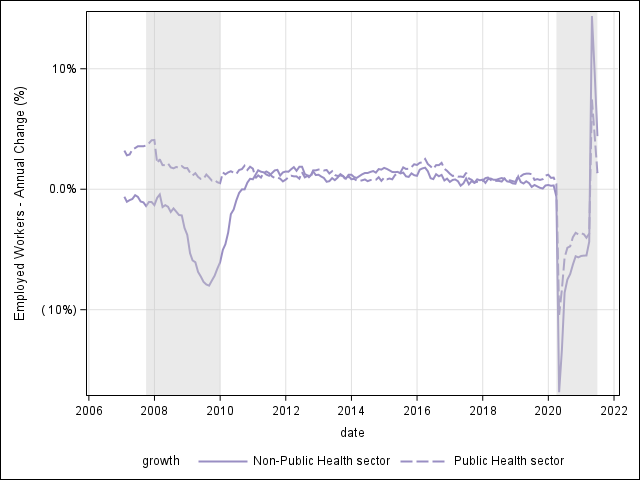
\includegraphics[scale = 0.9]{ohphs_vs_nonohphs_yoy_growth}

\begin{figure}[h]
\caption{Healthcare vs Non-Healthcare sectors in Ohio}
\vskip .1cm
\centering
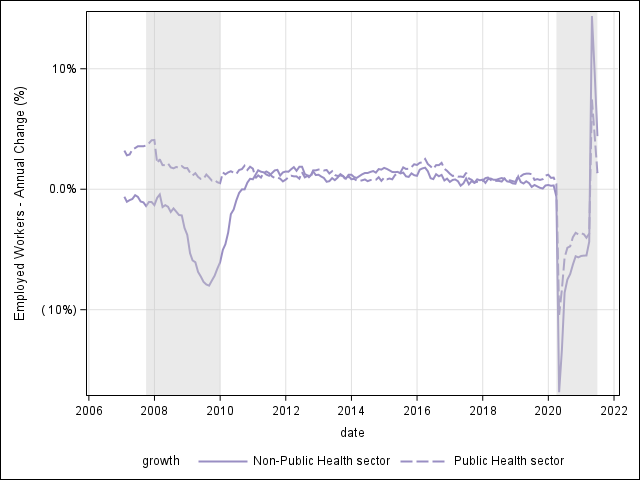
\includegraphics[scale = 0.9]{ohphs_vs_nonohphs_yoy_growth}
\end{figure}

The above figure shows year-over-year percentage change in number of employed workers in healthcare and non-healthcare sectors in Ohio. As seen above, the healthcare sector employment levels did not fall greatly during The Great Recession, even though other sectors saw a significant reduction in job levels. Contrastingly, COVID-19 recession led to a sharp reduction in healthcare workforce and this decline mimicked the reduction in non-healthcare sectors, although the decline in healthcare was not as steep. 


The unit-level data allows us to look further than just observing aggregate employment patterns and observe more deeply how people may be affected by the changing state of the economy. Whenever a representative unit hires a new person and adds them to their payroll, a new job is created and whenever a person is removed from the payroll, a job is destroyed. Even within Ohio, thousands of jobs are added and destroyed every day. These new jobs can either be created by existing firms which are expanding their workforce or by new firms entering the market. Analyzing the number of jobs created by new and existing firms in Ohio can tell us how likely is a person to get a job. Similarly, when firms downsize their workforce or exit the market, they destroy jobs. Analyzing the number of jobs destroyed by surviving and exiting firms in Ohio can tell us how likely a person is to lose a job. Together, these variables can tell us about the ongoing shifts in the labor markets. 


\section{Methodology} \label{s:methods}

{\bf Data}

\noindent
The data for this study comes from Ohio Department of Job and Family Services (OJFS) and ranges from January 2006 to June 2021. Ohio Revised Code (ORC) Section 4141.13 (G) requires the OJFS to collect information from all Ohio employers to determine if they are subject to the state’s unemployment insurance laws. According to OJFS website \cite{ui}, unemployment benefits are financed by taxes paid by employers to the federal and state governments. The federal taxes cover most of the program’s administrative costs and the state taxes fund the actual benefits. Unemployment benefits provide short-term income to workers who lose their jobs through no fault of their own and who are actively seeking work. OJFS collects this data via their State of Ohio Unemployment Resource for Claimants and Employers (SOURCE) application. The employers report to OJFS the number of employees on their payroll every month and the wages paid to the employees. Each employer has a unique Employer Identification Number (EIN) and is classified as per North American Industry Classification system (NAICS). 

Now, we define the NAICS category and major Healthcare subcategories considered for this study. NAICS records category 62 as healthcare and social assistance \cite{naicspdf}. One important thing to note is that NAICS does not distinguish between healthcare and social assistance services, citing difficulties in identifying the boundaries of these activities. We follow the same delineation and consider the four highest categories under this sector: Ambulatory Healthcare (621), Hospitals (622), Nursing and Residential care (623) and Social Assistance (624).  
\\

Ambulatory Healthcare sector servers patients who do not require inpatient services and are generally associated with outpatient services i.e. they do not require the patient to be admitted overnight. Offices of Physicians, dentists, optometrists, mental health practitioners, occupational \& speech therapists and outpatient care centres fall under this category.

Hospitals form the majority of the healthcare sector and mainly provide medical, diagnostic and treatment services to inpatients but can also have small-scale outpatient services. These healthcare institutions are generally much larger in size than units under other sectors and provide specialized facilities that are essential for the region.

Nursing and residential care sector provides nursing, supervisory, residential or any other type of care required by its patients, who are sometimes referred as residents.

Social assistance sector provides a wide variety of social assistance services directly to their clients which include but are not limited to individual and family services, childcare services, community food services and temporary shelters \& housing services.

\vskip .2cm

{\bf Variables}

\noindent
1.	Number of employed persons is the variable of interest and is defined as the number of workers that were reported to OJFS by a unit and were part of its payroll

\noindent
2.	NAICS code variable identifies the specific industrial category of a unit as per North American Industry Classification System

\noindent
3.	Sub-categories variable uses NAICS code and separates sectors into healthcare and non-healthcare

\noindent
4.	Unique location identifier, known as “unit” throughout this paper, was used to identify a particular location or address related to healthcare sector

\vskip .2cm

{\bf Measures}

\noindent
In order to truly understand the jobs related to Ohio’s healthcare sector, we need to study the dynamics of the Ohio’s healthcare labor market. In this paper, we do this by analyzing job flows, that is, the creation and destruction of jobs within the healthcare sector, and its subsectors. 
Job creation rate represents the sum of job gains measured at a unit over one month due to either opening of new units or expansion of jobs within an existing unit.
Job destruction rate represents the sum of job losses resulting from either closing of a production unit or contraction in the number of jobs by an existing unit. 
Job reallocation rate is equal to the sum of job creation rate and job destruction rate.
Net employment rate is equal to the difference between job creation rate and job destruction rate.
All the rates were based on monthly data and were calculated on an annual or year-over-year basis.
Below, we mathematically define each of these measures.
\\
\\
Let $E_{it}$ be defined as the number of people on $i^{th}$ company's payroll during $t^{th}$ time period, where $i \in \{1, 2, .... , N \}$ for some $N \in \N $ and $t \in \{1,2, ...., T\}$ for some $T \in \N$
\\
Then, 
\vskip 0.1cm
Let monthly job creation be $JC_t = \frac{1}{N} \sum_{i=1}^{N} JC_{it}$, where

\[
JC_{it}=\begin{cases} E_{it} - E_{it-1}  &\text{, if } E_{it} - E_{it-1} \ge 0 ,\\ 0 &\text{, if } E_{it} - E_{it-1} < 0 \end{cases}
\]
\vskip 0.2cm
Let monthly job destruction be $JD_t = \frac{1}{N} \sum_{i=1}^{N} JD_{it}$, where

\[
JD_{it}=\begin{cases} 0  &\text{, if } E_{it} - E_{it-1} \ge 0 ,\\ -(E_{it} - E_{it-1}) &\text{, if } E_{it} - E_{it-1} < 0 \end{cases}
\]
\vskip 0.2cm
Let annual Job creation rate be $JCR_t = \frac{JC_t}{\sum_{i=1}^{N} E_{it}}  - \frac{JC_{t-12}}{\sum_{i=1}^{N} E_{it-12}} $ 
\vskip 0.3cm
Let annual Job destruction rate be $JDR_t = \frac{JD_t}{\sum_{i=1}^{N} E_{it}}  - \frac{JD_{t-12}}{\sum_{i=1}^{N} E_{it-12}} $
\vskip 0.3cm
Let Reallocation rate be $RR_t = JCR_t + JDR_t$ 
\vskip 0.2cm
Let Net Employment rate be $NER_t = JCR_t - JDR_t$ 
\vskip 0.2cm

\pagebreak

\section{Results} \label{s:results}

We first share the results related to jobs generated by each subsector within healthcare before and after COVID. Post COVID period begins April 2022, after the announcement of stay-at-home order by ODH.

\begin{figure}[h]
\caption{Ohio Healthcare sector: Jobs generated per NAICS category}
\vskip .1cm
\centering
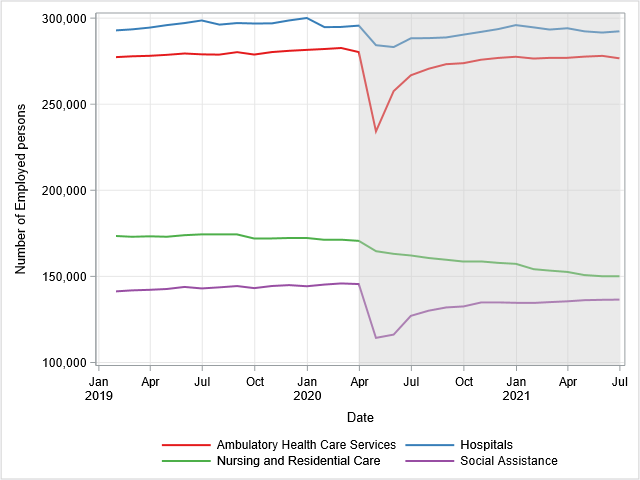
\includegraphics[scale = 0.9]{ts_ohphs_empl_by_subcat_mth}
\label{fig:jobs}
\end{figure}


Figure \ref{fig:jobs} shows monthly number of employed persons within Ohio by each major NAICS subsector under healthcare. All subsectors experienced a decline due to lockdown imposed by COVID-19, but the sharpest decline was experienced by Ambulatory Health Care Services and Social Assistance sectors. Both these sectors recovered after the shock, but have so far failed to reach the pre-COVID levels. Hospitals experienced a temporary decline but also recovered promptly. Nursing sector has experienced a constant decline since the advent of COVID crisis.

\vskip 0.5cm

\begin{table}[h]
\caption{Job Creation \& Destruction Flows as a percentage of total employment}
\resizebox{\textwidth}{!}
{
\begin{tabular}{llccccc}
\hline
\rowcolor[HTML]{C0C0C0} 
Category & Period & Job Creation & Job Destruction & Job Reallocation & Net Employment  \\ \hline
Ambulatory Healthcare & Pre-COVID & 3.26\% & 3.11\% & 6.38\% & 0.15\%  \\ \hline
Ambulatory Healthcare & Post-COVID & 3.88\% & 4.15\% & 8.02\% & (0.27\%) \\ \hline
Hospitals & Pre-COVID & 1.09\% & 1.01\% & 2.11\% & 0.08\% \\ \hline
Hospitals & Post-COVID & 1.13\% & 1.19\% & 2.33\% & (0.06\%) \\ \hline
Nursing and Residential Care & Pre-COVID & 2.53\% & 2.52\% & 5.05\% & 0.01\% \\ \hline
Nursing and Residential Care & Post-COVID & 2.84\% & 3.68\% & 6.52\% & (0.83\%) \\ \hline
Social Assistance & Pre-COVID & 3.45\% & 3.17\% & 6.62\% & 0.28\% \\ \hline
Social Assistance & Post-COVID & 4.19\% & 4.84\% & 9.03\% & (0.64\%) \\ \hline
Healthcare Sector & Pre-COVID & 2.39\% & 2.27\% & 4.66\% & 0.12\% \\ \hline
Healthcare Sector & Post-COVID & 2.77\% & 3.10\% & 5.87\% & (0.33\%) \\ \hline
\end{tabular}
}
\label{table:ohphscovid}
\end{table}
\vskip 0.2cm
Table \ref{table:ohphscovid} shows average pre and post COVID-19 lockdown levels for job creation, destruction, reallocation and net employment rates for healthcare and its subsectors. Pre COVID period is up to March 2020 and post COVID period begins April 2020 i.e. once the stay-at-home order was announced. 
Each sector had a positive net employment rate before COVID but has a negative net employment rate after COVID. For example, Ambulatory Healthcare sector had a net employment rate of $0.15\%$ before COVID but had a net employment rate of $-0.27\%$ after COVID.

\noindent
All sectors had a higher job creation rate post COVID than pre COVID. Similarly, all sectors had a higher job destruction rate post COVID than pre COVID. However, the difference between job destruction rate before and after COVID was much higher than the difference between job creation rate before and after COVID. For instance, Social Assistance sector had a pre COVID job creation rate of $3.45\%$ and a post COVID job creation rate of $4.19\%$ which lead to an increase of $0.74$ percentage points (pp). Similarly, it had a pre COVID job destruction rate of $3.17\%$ and a post COVID job destruction rate of $4.84\%$ resulting in an increase of $1.67$ pp. Note that job destruction rate between the two periods is more than double the job creation rate. In other words, the difference between $1.67$ pp and $0.74$ pp is $0.93$, and this number is our measure of jobs lost in Social Assistance sector due to COVID-19. This difference measure reveals that newer jobs created after the advent of COVID-imposed restrictions were not able to fully compensate for the jobs destroyed by COVID-imposed restrictions. In this way, when we compute difference measures for all the healthcare subsectors provided in table \ref{table:ohphscovid}, we find that none of the sectors have been able to recover from the high job destruction rate caused by COVID-19.

\noindent
All sectors also had a higher job reallocation rate post COVID than pre COVID, which suggests that healthcare workers were more likely to switch their jobs after Ohio declared state of emergency due to COVID.


	
\section{Discussion} \label{s:discussion}

COVID recession was different from The Great Recession in terms of its impact on the healthcare sector. While other sectors in Ohio experienced a decrease in workforce during The Great Recession, healthcare and social assistance sector experienced no such decline. However, COVID had a very similar on both these broad sectors as all employers were forced to take safety measures.
COVID-19 also had a dissimilar impact on different healthcare sub-sectors.
Ambulatory healthcare sector experienced the sharpest decline due to lockdown imposed by COVID-19. This seems reasonable given that all outpatient services were temporarily halted by the stay-at-home order imposed by Ohio’s department of health. Soon after the stay-at-home order was lifted, the sector recovered from the temporary shock as units in this sector were allowed to reopen, albeit with COVID restrictions and policies in place.
Hospitals were the most stable and were least impacted, atleast in terms of payroll jobs, out of all healthcare subcategories as they were allowed to operate during the lockdown. The relatively small decline in this sector can possibly be attributed to closure of certain non-essential services or increased COVID-19 spread forcing the workers stay at home and as a result, out of the payroll system. On the other hand, one would imagine that hospitals should have experienced a surge in new workforce as there were cases of extreme labor market tightening during the pandemic. However, even when they were the most important institutions during the pandemic, hospitals experienced a moderate decline in net employment rate.
Social Assistance sector had an average post COVID job reallocation rate of $9\%$ and was the highest among the healthcare subsectors, along with the highest gap between job destruction and job creation rates. This suggests a lot of movement of healthcare workers away from this sector, as a number of people in this sector were laid off during lockdown and had to find other jobs. 
Nursing sector had the lowest post COVID net employment rate and is experiencing a continuous decline in workforce. This suggests a deeper problem than a one-time shock. One possible explanation is the decline in demand of such services due to shift in demographics caused by COVID-19. Because the elderly and the disabled were disproportionately affected by COVID-19, this possibly resulted in a higher death rate among these groups and ultimately led to a lower demand for nursing and residential care facilities. 


\section{Public Health Implications}\label{s:implications}

Healthcare sector in Ohio experienced tremendous increase in labor market activity due to the effect of COVID-19 and stay-at-home order issued in March 2020. New jobs were created throughout the healthcare industry as demand for telehealth, telemedicine and COVID-related healthcare services increased employment levels. However, this demand was more than offset by the decrease in jobs at some of the existing healthcare institutions, as they were forced to cut costs by eliminating non-essential services from their payrolls. Contrary to the common misconception that healthcare sector is expanding due to increased demand for healthcare workers caused by COVID-19, the payroll data from OJFS shows us a decrease in overall healthcare employment as of June 2021. In the future, some sectors such as Hospitals may create new jobs as they seem to have relatively stable job creation and destruction rates, whereas other sectors such as Nursing and Residential Care may be on their way towards permanent decline in job opportunities. 



\if0\blind{
\section*{Acknowledgements}
This project was supported by Wolfgang Mayer Fellowship provided by University of Cincinnati. We acknowledge and thank Dr. Michael Jones, Professor at University of Cincinnati, for his help with procurement of data. The data was provided via quarterly csv files uploaded by Office of Workforce Development at Ohio JFS on Axway Server maintained by the department. The opinions, findings, and conclusions expressed in this publication are those of the author and do not necessarily reflect the official views of any other parties involved. To assess the quality of the data used in this study, OJFS payroll data was benchmarked against BLS employment data for healthcare sector . This comparison confirmed the quality of data and the benchmarking analysis is available upon request.	} \fi

\bibliographystyle{apacite}
% \spacingset{1}
\bibliography{IISE-Trans.bib}
	
\end{document}
